\lecture{3}{Oct 4 2024 Fri (13:00:10)}{Axiom of Completeness}

The defining difference between $\R$ and $\Q$ is that $\R$ does not contain the gaps that permeate $\Q$. We will be precise about how we phrase this assumption. This is referred to as the \emph{Axiom of Completeness}.
\begin{frame}[Axiom of Completeness]
  \begin{center}
    Every nonempty set of real numbers that is bounded above has a least upper bound.
  \end{center}
\end{frame}

\begin{note}
  We will never be able to prove the Axiom of Completeness, as axioms are meant to be taken as true. However, this will be the only statement that we naively accept without any rigorous proof. Everything else will be proven from this axiom.
\end{note}

Now, let's break down the definition of the least upper bound.

\subsection{Least Upper Bound and Greatest Lower Bound}

\begin{definition}[Upper Bound]
  A set $A \subseteq \R$ is bounded above if $(\exists b \in \R)(\forall a \in A)[a \le b]$. The number $b$ is called the \emph{upper bound} for $A$.
\end{definition}

\begin{definition}[Least Upper Bound]
  A real number $s$ is the \emph{least upper bound} for a set $A \subseteq \R$ if it meets the following two criteria
  \begin{enumerate}
    \item $s$ is an upper bound for $A$.

    \item If $b$ is any upper bound for $A$, then $s \le b$.
  \end{enumerate}
\end{definition}

\begin{example}
  Take the set $A = [-M, M]$. Then, all the numbers $m \ge M$ are upper bounds for $A$, while, only $M$ is the least upper bound.
\end{example}

The least upper bound is also called the \emph{supremum} of the set $A$. The \emph{greatest lower bound}/\emph{infimum} for $A$ is also defined similarly (see the figure below for a graphical representation).
\begin{figure}[H]
  \centering

  \begin{tikzpicture}[scale=0.9]
    \draw[thick] (-7, 0) -- (7, 0);

    % lower bounds from -6.8 to -2.4
    \draw[decorate,decoration={mirror,brace,amplitude=5pt},thick] (-6.8, -0.4) -- (-2.4, -0.4) node[midway, below=5pt] {lower bounds};

    % The set A from -2.2 to 2.2
    \draw[thick,fill=black] (-2.2, 0) -- (-2.2, 0.15) -- (-1.2, 0.15) -- (-1.2, 0) -- cycle;
    \node[above=15pt] (Inf) at (-2.2,0.15) {$\inf(A)$};
    \node[above=1pt] (Box1) at (-2.2,0) {};
    \draw[arrows={->}] (Inf) edge (Box1);

    \draw[thick,fill=black] (-0.8, 0) -- (-0.8, 0.15) -- (0.8, 0.15) -- (0.8, 0) -- cycle;

    \draw[soldot] (2.2,0.07) circle (0.08);
    \draw[soldot] (2.1,0.07) circle (0.08);
    \draw[soldot] (1.95,0.07) circle (0.08);
    \draw[soldot] (1.75,0.07) circle (0.08);
    \draw[soldot] (1.5,0.07) circle (0.08);
    \draw[soldot] (1.2,0.07) circle (0.08);

    \node[above=15pt] (Sup) at (2.2,0.15) {$\sup(A)$};
    \node[above=1pt] (Box2) at (2.2,0) {};
    \draw [arrows={->}] (Sup) edge (Box2);

    \node[below=5pt] (A) at (0,-0.4) {$A$};
    \node[below=1pt] (O) at (0,0.2) {};
    \draw[arrows={->}] (A) edge (O);

    \node[below=1pt] (AE1) at (-1.7,0.2) {};
    \draw[->] (A.west) -- (AE1);

    \node[below=1pt] (AE2) at (1.7,0.2) {};
    \draw[->] (A.east) -- (AE2);

    % upper bounds from 2.2 to 6.8
    \draw[decorate,decoration={mirror,brace,amplitude=5pt},thick] (2.2, -0.4) -- (6.8, -0.4) node[midway, below=5pt] {upper bounds};
  \end{tikzpicture}
\end{figure}

\begin{notation}
  The supremum is denoted as $s = \sup(A)$ and the infimum is denoted as $s = \inf(A)$.
\end{notation}

\begin{claim}
  A set that's bounded can only have one least upper bound.
\end{claim}

\begin{proof}
  By property (ii) of the definition of the least upper bound, if $s$ and $t$ are both least upper bounds for $A$, then $s \le t$ and $t \le s$, implying that $s = t$.
\end{proof}

\begin{example}
  The closed interval $[a, b]$ has a supremum of $b$ and an infimum of $a$. So does the open interval $(a, b)$. But what's the difference between the two? We'll investigate that later on.
\end{example}

\begin{example}
  Let $A = \left.\left\{\frac{1}{n}~\right\rvert n \in \N\right\} = \left\{1, \frac{1}{2}, \frac{1}{3}, \dots\right\}$. It's clear that $\sup(A) = 1$ and $\inf(A) = 0$.
\end{example}

\subsection{Maximum and Minimum}

\begin{definition}[Maximum and Minimum]
  A real number $a_0$ is a \emph{maximum} of the set $A$ if $a_0$ is an element of $A$ and $(\forall a \in A)[a_0 \ge a]$. Similarly, $a_0$ is a \emph{minimum} of the set $A$ if $a_0$ is an element of $A$ and $(\forall a \in A)[a_0 \le a]$.
\end{definition}

The closed interval $[a, b]$ has a maximum of $b$ and a minimum of $a$, since they're both elements of the set. However, the open interval $(a, b)$ has neither a maximum nor a minimum, since $a$ and $b$ aren't in the set.

\begin{example}
  Let $A = \left.\left\{1 + \frac{1}{n}~\right\rvert n \in \N\right\}$, giving us $\sup(A) = 2 = \max(A)$, but $\inf(A) = 1 \ne \min(A)$, as it does not exist.
\end{example}

\begin{question}
  Let $A \subseteq \R$ be nonempty and bounded above, let $c \in \R$. Define the set $c + A = \left\{c + a \mid a \in A\right\}$. Then, $\sup(c + A) = c + \sup(A)$.
\end{question}

\begin{proof}[Solution]
  Let $s = \sup(A)$. Let $a \in A$. Since $s$ is an upper bound of $A$, then $a \le s \implies a + c \le s + c$ implies that $c + s$ is an upper bound of $c + A$. Then, $a \le s \implies a + c \le s + c \implies c + s$ is an upper bound of $c + A$. If $b$ is an upper bound of $A$, then $s \le b$. Now, let $d$ be an upper bound of $c + A$. Then, $c + a \le d \implies a \le d - c \iff d - c$ is an upper bound of $A$. Then,
  \begin{align*}
    \phantom{\implies}\quad&s = \sup(A) \le d - c \\
    \implies\quad&s + c \le d \\
    \implies\quad&s + c = \sup(c + A)
  .\qedhere\end{align*}
\end{proof}

\subsection{Proving the upper bound}

How do we actually show that $a$ is an upper bound for a set $A \subseteq \R$? We use the following
\begin{lemma}
  Assume $s \in \R$ is an upper bound for a set $A \subseteq \R$. Then, $s = \sup(A)$ if and only if, $(\forall \epsilon > 0)(\exists a \in A)[s - \epsilon < a]$.
\end{lemma}

\begin{proof}
  Assume $s = \sup(A)$. Let $\epsilon > 0$. Then $s - \epsilon < s$, implying that $s - \epsilon$ is not an upper bound for $A$. Then, there must exist some $a \in A$ such that $s - \epsilon < a$, because otherwise, $s - \epsilon$ would be an upper bound.

  Assume $b$ is an upper bound for $A$. Assume $b < s \iff s - b > 0$. Let $\epsilon = s - b$. Then, $(\exists a \in A)[(s - \epsilon < a \iff b < a)]$, which is a contradiction, since $b$ is an upper bound. Therefore, $s = \sup(A)$.
\end{proof}

\begin{example}[Applying the Lemma]
  Let $A = \{1 - \frac{1}{n} : n \in \N\}$. We suspect $\sup(A) = 1$.
  \begin{enumerate}
    \item \textbf{Check upper bound:} For every $n$, $1 - \frac{1}{n} < 1$, so $1$ is an upper bound.

    \item \textbf{Check $\epsilon$-condition:} Given $\epsilon > 0$, choose $n$ such that $\frac{1}{n} < \epsilon$ (possible by the Archimedean property). Then $a = 1 - \frac{1}{n} \in A$ and
    \[
      s - \epsilon = 1 - \epsilon < 1 - \frac{1}{n} = a.
    \]
    Therefore, the lemma confirms $\sup(A) = 1$. \qedhere
  \end{enumerate}
\end{example}

\begin{example}[Supremum not in the Set]
  Consider $B = (0, 2) \cap \Q$. The set is bounded above by $2$. We claim $\sup(B) = 2$.
  \begin{itemize}
    \item $2$ is an upper bound.

    \item Given $\epsilon > 0$, choose $q \in \Q$ such that $2 - \epsilon < q < 2$ (possible since rationals are dense in $\R$). Then $q \in B$ and $2 - \epsilon < q$.

    \item The lemma ensures $\sup(B) = 2$ even though $2 \notin B$. \qedhere
  \end{itemize}
\end{example}

\begin{note}
  This $\epsilon$-characterization also works for $\inf(A)$ with signs flipped:
  \[%
    t = \inf(A) \iff [t~\text{is a lower bound and}~(\forall \epsilon > 0)(\exists a \in A)[a < t + \epsilon]]
  .\]%
\end{note}

\begin{example}[Non-Example]
  Let $C = \{x \in \R : x^2 < 2\}$. The number $s = 1.4$ is an upper bound for $C$ (since $1.4^2 = 1.96 < 2$). However, $s$ is not the supremum, because for $\epsilon = 0.05$, we can find $c \in C$ such that $1.4 + \epsilon = 1.45$ is still in $C$, contradicting $1.4$ being an upper bound. The real supremum is $\sqrt{2}$.
\end{example}

\subsection{Nested Interval Property}

\begin{theorem}[Nested Interval Property]
  For each $n \in \N$, assume we are given a closed interval $I_n = [a_n, b_n] = \left\{x \in \R \mid a_n \le x \le b_n\right\}$. Assume also that each $I_n$ contains the next interval, i.e., $I_n \supseteq I_{n+1}$. Then, the resulting sequence of closed intervals
  \[%
    I_1 \supseteq I_2 \supseteq I_3 \supseteq \cdots
  ,\]%
  has a nonempty intersection. That is,
  \[%
    \bigcap_{n=1}^\infty I_n \neq \emptyset
  .\]%
\end{theorem}

\begin{proof}
  Let $A = \{a_n : n \in \N\}$. Since $I_n \supseteq I_{n+1}$, we have $a_1 \le a_2 \le a_3 \le \cdots$ (the left endpoints are nondecreasing) and $b_1 \ge b_2 \ge b_3 \ge \cdots$ (the right endpoints are nonincreasing). Moreover, for each $n$ we have $a_n \le b_n \le b_1$, so $A$ is bounded above by $b_1$.

  By the Axiom of Completeness, $A$ has a least upper bound $s = \sup(A)$. Combining these inequalities, for every $n$ we have
  \[%
    a_n \le s \le b_n
  ,\]%
  which means $s \in I_n$ for all $n \in \N$. Hence
  \[%
    s \in \bigcap_{n=1}^\infty I_n
  ,\]%
  proving that the intersection is nonempty.
\end{proof}

The Nested Interval Property can be viewed graphically, as shown below.
\begin{figure}[H]
  \centering

  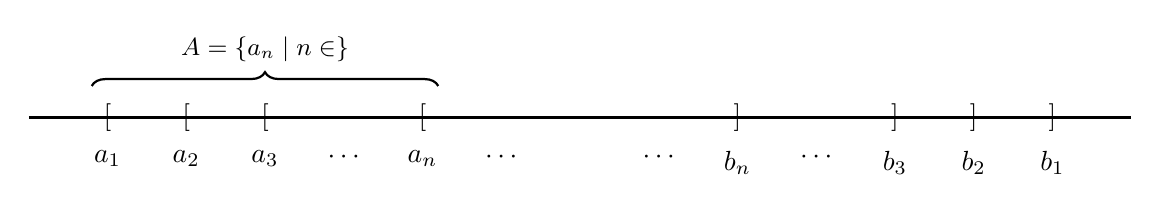
\begin{tikzpicture}
    \draw[thick] (-7, 0) -- (7, 0);

    \foreach \i/\pos in {1/-6, 2/-5, 3/-4, n/-2} {
      \node at (\pos, 0) {$[$};
      \node[below] at (\pos, -0.3) {$a_{\i}$};
    }
    \node[below] at (-3, -0.3) {$\cdots$};

    \foreach \i/\pos in {n/2, 3/4, 2/5, 1/6} {
      \node at (\pos, 0) {$]$};
      \node[below] at (\pos, -0.3) {$b_{\i}$};
    }
    \node[below] at (3, -0.3) {$\cdots$};

    \node[below] at (1, -0.3) {$\cdots$};
    \node[below] at (-1, -0.3) {$\cdots$};

    \draw[decorate,decoration={brace,amplitude=5pt},thick] (-6.2, 0.4) -- (-1.8, 0.4) node[midway, above=5pt] {{\small$A = \{a_n \mid n \in \N\}$}};
  \end{tikzpicture}
\end{figure}

\begin{example}\leavevmode
  \begin{enumerate}
    \item The interval $I_n = \left[0, \frac{1}{n}\right]$, which is clearly $I_n \supset I_{n+1}$, since $\bigcap_{n=1}^\infty = \{0\}$.

    \item The counter example is $I_n = \left(0, \frac{1}{n}\right)$, $\bigcap_{n=0}^\infty I_n = \emptyset$, since $0 \notin I_n$. \qedhere
  \end{enumerate}
\end{example}


\begin{proposition}
  The set $\N$ is unbounded.
\end{proposition}

\begin{proof}
  Assume, for contradiction, that $\N$ is bounded above. Then, it follows that we can set $\alpha = \sup(\N)$. If we consider $\alpha - 1$, then we no longer have an upper bound for $\N$, and therefore, there exists an $n \in \N$ satisfying $\alpha - 1 < n$, which is equivalent to $\alpha < n + 1$. Since we have $n + 1 \in \N$, this contradicts the assumption that $\alpha$ is the least upper bound of $\N$.
\end{proof}

\begin{theorem}[Archimedian Property]\leavevmode
  \begin{enumerate}
    \item $(\forall x \in \R)(\exists n \in \N)[n > x]$.

    \item $(\forall y > 0)(\exists n \in \N)[\sfrac{1}{n} < 1]$.
  \end{enumerate}
\end{theorem}

\begin{proof}\leavevmode
  \begin{enumerate}
    \item Property (i) follows given that $\N$ is unbounded.

    \item Apply property (i) with $x = \sfrac{1}{y} > 0$. \qedhere
  \end{enumerate}
\end{proof}
